\section{Implementation}
\label{sec:implementation}

This section first presents the architecture of the coDoc prototype tool, which implements our traceability link management framework. After that, we introduce the algorithms for validating the traceability links and for code selection completion which helps users to complete code piece selection when part of a syntax element is selected.

\subsection{Architecture}

The architecture of our approach is shown in Figure \ref{fig:architecture}.
There are three types of data here, 1) code, 2) spec, and 3) traceability links.
These data are consumed by three components: code manager (CM), spec manager (SM) and link manager (LM).
\begin{figure}
\begin{center}
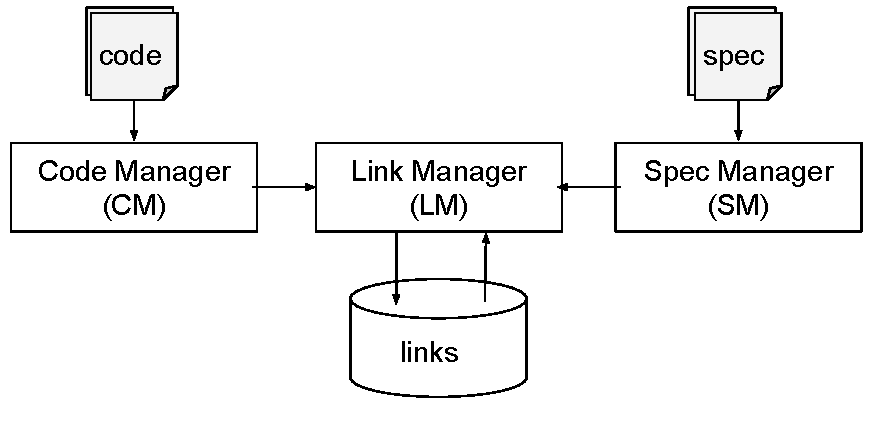
\includegraphics[width=0.55\textwidth]{architecture}
\caption{coDoc Architecture and Features}
\label{fig:architecture}
\end{center}
\end{figure}
\begin{enumerate}
\item \textit{Link Manager.} Traceability link manager gets the highlighted code piece from code manager and the highlighted spec piece from spec manager, and creates traceability link for these two piece of information. It also reads the traceability link data, verifies the validity of the link,
and highlights the code and document pieces that are related.
\item \textit{Code Manager.} Code manager reuses C/C++ Development Tool (CDT) editor from Eclipse~\cite{Eclipse} to parses the code,
and highlights syntax elements. It can highlight the piece of code based on the information provided by the user or the link manager.
\item \textit{Spec Manager.} Spec manager renders the pdf content, can support select and highlight spec content, and communicate with the link manager.
\end{enumerate}

We implemented coDoc as an Elipse Rich Client Program (RCP),
which can make our tool share the appearance in Eclipse that is familiar by many programmer.
Figure \ref{fig:platformview} is the screenshot of the tool.
The bottom is the UI for link manager, while the top middle part and top right side are the UI for code manager and spec manager respectively.
To traverse a traceability link, users can select a link from the list in the link manager or click on a code construct in the code manager. 
As a result, the link, the relevant code, and the relevant spec piece are highlighted in the link, code, and the spec mangers. 

% convert platformview.png platformview.eps
\begin{figure}
\begin{center}
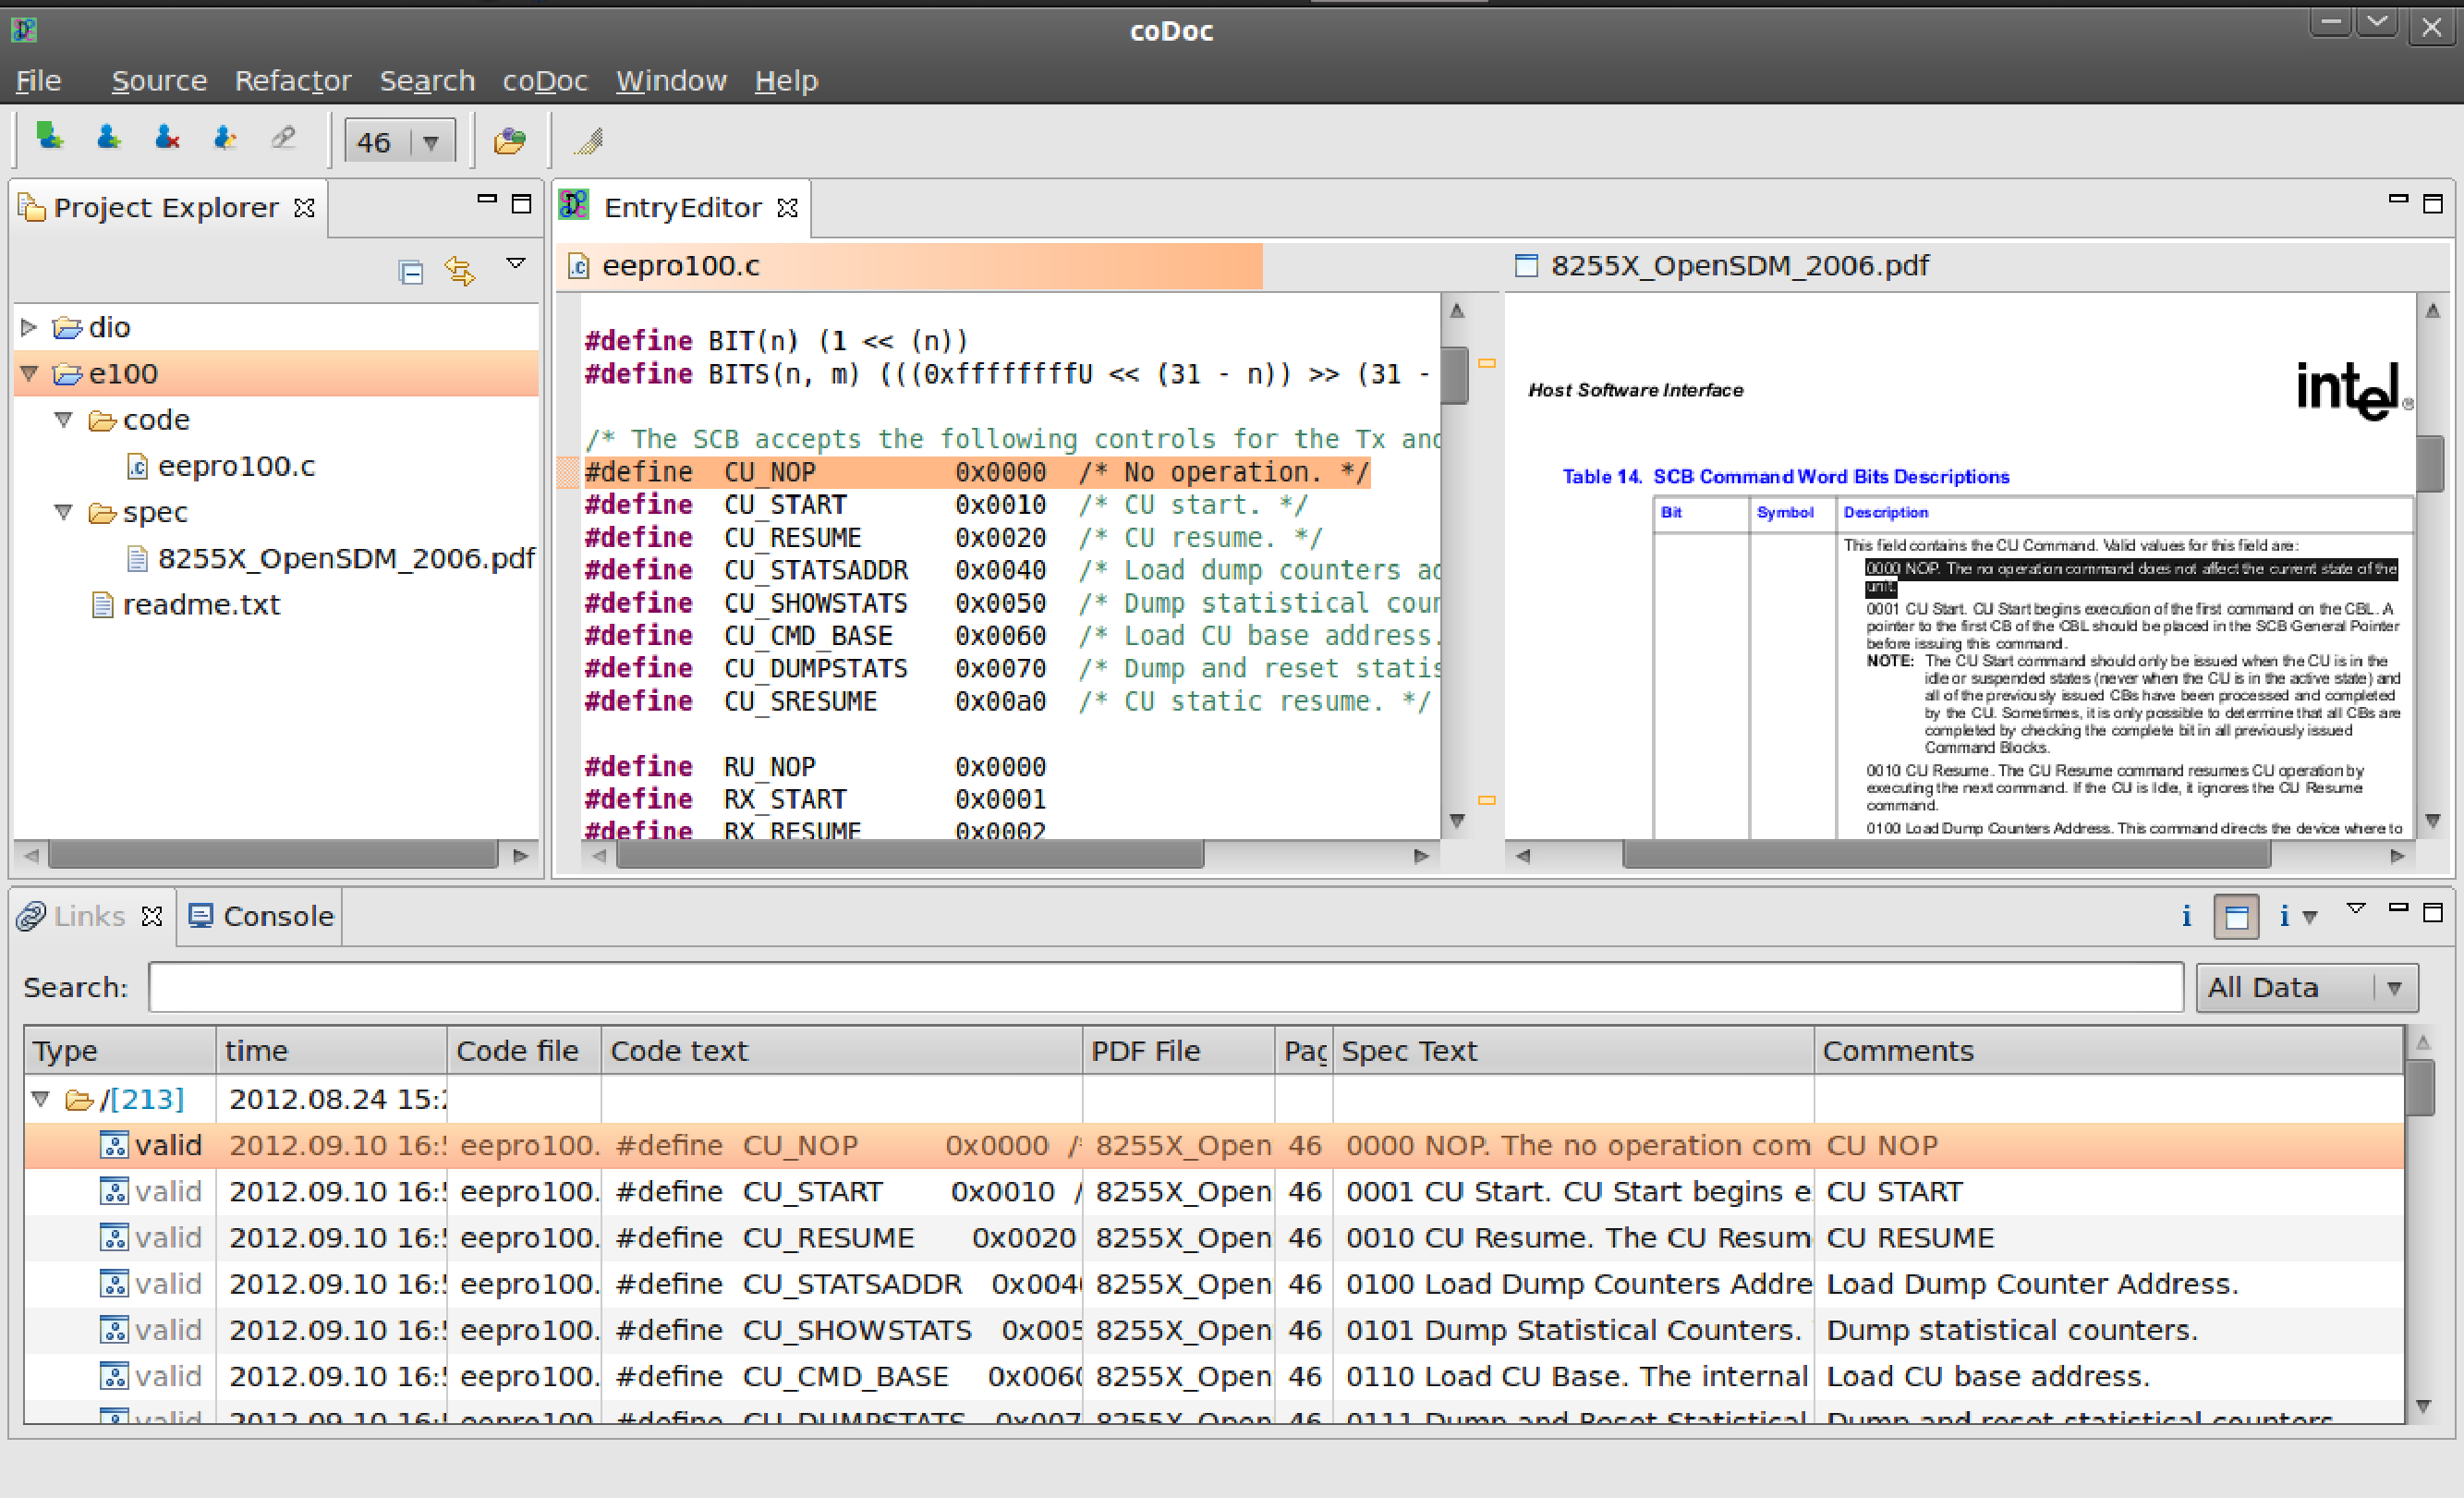
\includegraphics[width=\textwidth]{platformview}
\caption{coDoc User Interface Screenshot}
\label{fig:platformview}
\end{center}
\end{figure}


\subsection{Link Validation}

%\begin{figure}[h!]
%  \begin{center}
%    \begin{minipage}[b]{0.6\linewidth}
%      \centering
%      \renewcommand{\ttdefault}{pcr}
%      \begin{lstlisting}
%for each leaf node in syntax tree
%  for each node in anchor
%    node string compare
%\end{lstlisting}
%\end{minipage}
%\caption{Pseudocode for Link Validation}
%\label{fig:validate}
%\end{center}
%\end{figure}

When code evolves, we need to validate the existing traceability links.
Once an invalid traceability link is found, we report it and ask the user to correct it manually.
To check the validity of the traceability links, we record the content of the code piece and the spec piece when generating the links.
The content is used later to compare with the content to which the path points to when code changes.
The validation process basically goes through each traceability link in the database,
and checks whether the link is valid or not.
\begin{algorithm}[!h]
\DontPrintSemicolon
\SetKwComment{tcp}{\hfill$\triangleright$ }{}
\SetCommentSty{emph}
$AST \leftarrow \textsc{Gen-AST}(code)$\;
$\langle RES, CONTENT_C \rangle \leftarrow \textsc{Get-Code-Content}(AST, link.code.path)$\;
\If{$RES = FALSE$} {
\Return $FAILURE$\;
}
$RES \leftarrow \textsc{Compare-Content}(CONTENT_C, link.code.content)$\;
\If{$RES = FAIL$} {
\Return $FAILURE$\;
}
$CONTENT_S \leftarrow \textsc{Get-Spec-Content}(spec, link.spec.path)$\;
$RES \leftarrow \textsc{Compare-Content}(CONTENT_S, link.spec.content)$\;
\If{$RES = FAIL$} {
\Return $FAILURE$\;
}
\Return $SUCCESS$\;
\caption{$\textsc{Traceability-Link-Validation}(link)$}
\label{alg:validate}
\end{algorithm}
Algorithm~\ref{alg:validate} presents the pseudo-code for check the validation of one single traceability link.
Line 1 - line 7 check the validity of the code piece part of the traceability link.
Line 1 generates the AST for the current code first.
Line 2 then invokes the function \textsc{Get-Code-Content} with the path of the code piece as input, identify the code piece in the new AST, and return the content of the code piece if the code piece is identified successfully.
If the path of the code piece cannot identify any code piece or can identify more than one code piece, the function \textsc{Get-Code-Content} reports failure.
Line 5 compares the the content extracted from the new code with the recorded content, and reports failure if they do not match.
After finishing checking the code piece, line 8 - line 11 of the algorithm check the spec piece in a similar flow.
If no failure happens, the algorithm returns successfully at line 12.


\subsection{Code Selection Completion}

%To improve the user experience of coDoc, we help users to select the code pieces when creating traceability links.
The coDoc tool assists user to select the code pieces that can be used in traceability links. Each code piece selected is required to be a complete language construct.
%Our approach is based on the fact that it is usually meaningless to have part of the basic code elements as the code piece of the traceability links.
For example, we do not create a link between part of a variable name in the code and part of a word in the spec.
We assume that every selected piece of code is composed of valid syntax elements.
Based on this assumption, we can help users to automatically complete their selection when they only select part of a syntax element such as a variable. 
Algorithm \ref{alg:completion} outlines our approach.
\begin{algorithm}[!h]
\DontPrintSemicolon
\SetKwComment{tcp}{\hfill$\triangleright$ }{}
\SetCommentSty{emph}
$AST \leftarrow \textsc{Gen-AST}(code)$\;
$LEAF\_SEQ \leftarrow \textsc{Gen-Leaf-Sequence}(AST)$\;
$AST\_selection \leftarrow \textsc{To-AST-Based}(LEAF\_SEQ, original\_offset)$\;
$new\_offset \leftarrow \textsc{To-Offset-Based}(AST\_selection)$\;
\Return $new\_offset$\;
\caption{$\textsc{Complete-Code-Selection}(orginal\_offset)$}
\label{alg:completion}
\end{algorithm}
This algorithm takes a code selection in the offset based format,
and returns a new, appropriately enlarged code selection in the offset based format.
We choose offset based format because Eclipse use this format to highlight code pieces.
The algorithm basically works as follows: (1) lines 1 - 3 align the input offset-based selection to its smallest enclosing language construct by analyzing the AST.
(2) line 4 maps the enlarged code selection to the offset based format and returns it.  
As we discussed above, the AST based selection is a sequence of AST leaf nodes in the depth-first-search order, which is the same order as the code in the source code.
The AST based code piece covers all the meaningful part of the original offset based code piece.
To transform the offset based selection to the AST based selection,
we obtain the sequence of leaf nodes of the AST in line 1 and line 2,
and then match the leaf node sequence with the offset-based selection to get the enlarged AST based selection.
The leaf nodes in the AST based selection is determined as follows: if a leaf node contains any part of the offset selected code, then the leaf node is in the AST based selection.
After we obtain the AST based selection, we transform it back to a new, enlarged offset based selection, and display it to users.
Each time users make a selection, coDoc adjusts the selection to valid syntax boundary.

